%% [ADS 4-2005] Template file for 40in x 30in landscape poster
%%
%%
%%
%%
%% [ADS 4-2005] what follows here is obsolete I believe.
%%-------------------------------------------------------------------------
%% Written by Graeme, 2001-03 based on Norman's original microlensing
%% poster.
%%
%% $Id: poster-template-landscape.tex,v 1.1 2001/07/02 17:23:32 norman Exp $
%%
%% Default mode is landscape, which is what we want, however dvips and
%% a0poster do not quite do the right thing, so we end up with text in
%% landscape style (wide and short) down a portrait page (narrow and
%% long). Printing this onto the a0 printer chops the right hand edge.
%% However, 'psnup' can save the day, reorienting the text so that the
%% poster prints lengthways down an a0 portrait bounding box.
%%
%% 'psnup -w85cm -h119cm -f poster_from_dvips.ps poster_in_landscape.ps'
%%
%%-------------------------------------------------------------------------
%% Modified by Ronald Kumon, 06-2002 to incorporate a framebox border,
%%   add acknowledgments line at bottom, and change locations of logos
%%
%% Modified by Anand D. Sarwate 04-2005 to specialize to the UC Berkeley 
%%   EECS Wireless Foundaions conference poster template and for different
%%   paper sizes


%% [ADS 4-2005] latex --> dvips --> ps2pdf works just fine for me.
%%
%% To preview using xdvi:
%% 
%% $ xdvi -paper 1188x840mm -s 24 -nopostscript poster.dvi
%%
%% To convert dvi to Postscript:
%%
%% $ dvips -Ppdf -G0 -o poster.ps poster.dvi
%%
%% The dvips options are:
%% Ppdf: use the PDF printer configuration file
%% G0  : shift lower characters to higher position 
%%       (splits ligatures when using Times-Roman font)
%%
%% To convert Postscript to PDF:
%%
%% $ pstill -c -giptCQ -w 3368 -h 2378 -o poster.pdf poster.ps
%% ($ pstill -c -iptCQ -w 3225 -h 2378 -o poster.pdf poster.ps)
%%
%% Note that the pstill options are
%% c:  compression (more c's give more compression; up to four)
%% g:  take size from Postscript file
%% p:  include all fonts as partial fonts
%% i:  include all non-standard fonts
%% t:  map graphics transfer functions from PostScript to PDF. 
%% C:  use RGB color map
%% w:  width in points (1/72 inch) for 1188 mm
%% h:  height in points (1/72 inch) for 839 mm
%% Q:  take embedded fonts from PSFonts directory, not Postscript file
%% Note also that the -w and -h options need to be included else
%% some of the Postscript figures may not be displayed (particularly
%% those converted using fig2dev), even if the -g option is specified.
%% Also, the newest version of pstill (1.55.91) does not deal well with 
%% slanted Times Roman font; use italics or the older version (1.55.3). 
%%-------------------------------------------------------------------------


\documentclass{article}
%% [ADS 4/2005]  The template here does NOT make use of the 'slides'
%% option of Kumon in the interest of creating a more readable document
%% -- suggestions for how to make a backup style on separate sheet is
%% given in the text.
%%

%% If you want to number equations, set the equation number counter to zero.
%\setcounter{secnumdepth}{0}









%%%%%%%%%%%%%%%%%%%%%%%%%
%%% PACKAGE INCLUSION %%%
%%%%%%%%%%%%%%%%%%%%%%%%%

%% AMS packages for special symbols, etc
% \usepackage{amsmath,amssymb}
\usepackage{amssymb,amsmath,amsthm}

%% This package gives you coloured text and various other simple
%% graphics hacks.  For details, see documentation in 
%% in /usr/local/teTeX/texmf/doc/generic/pstricks/*
\usepackage{pstricks}
\newrgbcolor{darkblue}{0.1 0.1 0.5}

%% The textpos package is necessary to position textblocks at arbitary 
%% places on the page.  Use showboxes option to show outlines of textboxes.
\usepackage[absolute]{textpos}
% \usepackage[absolute,showboxes]{textpos}

%% Package to include graphics.  
\usepackage{graphicx}
%% Define path for figures -- for safety, keep the last /
\graphicspath{{/your/figure/directory/here/if/any/}
{/an/second/directory/path/can/go/here/}}









% stuff I used

% to name equations
\newcommand{\eqname}[1]{\tag*{#1}}

%to remove the reference section title
\usepackage{natbib}
\renewcommand{\bibsection}{}

%for the algo
% \usepackage{algorithm}
% \usepackage[noend]{algpseudocode}

% \usepackage{graphicx}
% \usepackage{multirow,bigstrut}

% \usepackage[options]{algorithm2e}


% \usepackage[makeroom]{cancel}

\usepackage{algorithm}
% \usepackage{algorithmic}
\usepackage{caption}
\usepackage[noend]{algpseudocode}


% \usepackage{multirow,bigstrut}
% \usepackage{textcomp}









%% Wrap text around figures
%\usepackage{wrapfig}

%% Use Times font instead of Computer Modern -- this gives better
%% appearance when resizing to large sixes.
%% Note that without the ``G0'' in the dvips conversion, 
%% all character combinations that will normally result in 
%% ligatures will have to be hacked to display properly.  For example, 
%%     fi --> \mbox{f}\mbox{i}
%% Other characters may also fail.  In addition, the Mathtimes font 
%% set should really be used for mathematics, but unfortunately they 
%% are only proprietary.  (The Computer Modern fonts may still look OK.)
\usepackage{times}

%% These colors are tried and tested for titles and headers. Don't
%% over use color!
%\usepackage[usenames]{color} % commented by Karol Kozioł
\usepackage{xcolor}
\definecolor{DarkBlue}{rgb}{0.1,0.1,0.5}
\definecolor{Black}{rgb}{0.0,0.0,0.0}
\definecolor{Red}{rgb}{0.9,0.0,0.1}
\definecolor{DarkBlue2}{rgb}{0.00,0.08,0.6}
\definecolor{DarkRed2}{rgb}{0.6,0.00,0.08}
\definecolor{DarkGreen2}{rgb}{0.00,0.6,0.08}

%% Load shadow box package
%\usepackage{shadow}

%% This loads font sizes in style file a0size
\usepackage{a0size}





%%%%%%%%%%%%%%%%%%%%%%%%%%%%%%%% 
%%% NEW COMMAND DEFINTITIONS %%%
%%%%%%%%%%%%%%%%%%%%%%%%%%%%%%%%

%% See documentation for a0poster class for the size options here
%%    \normalsize will produce smaller type that might look too small
%%    \large will produce larger type
%% Feel free to modify if you want a different look

%SIZE OF TEXT
%doesnt seem to make a difference
\let\Textsize\normalsize
% \let\Textsize\large


\def\RHead#1{\noindent\hbox to \hsize{\hfil{\LARGE\color{DarkBlue} #1}}\bigskip}

\def\LHead#1{\noindent{\LARGE\color{DarkBlue} #1}\bigskip}

\def\CHead#1{\begin{center}\noindent{\LARGE\color{DarkBlue} #1}\end{center}}

\def\Subhead#1{\noindent{\large\color{DarkBlue} #1}\bigskip}

\def\Title#1{\noindent{\textsc{\textbf{\VeryHuge\color{DarkBlue} #1}}}}




%%%%%%%%%%%%%%%%%%%%%%%%%%%%%
%%% GLOBAL LAYOUT OPTIONS %%%
%%%   NUMBER OF COLUMNS   %%%
%%%%%%%%%%%%%%%%%%%%%%%%%%%%%

%% Set paper size
%% Depending on the conference, the posterboard size may be different.
%% This template was based on an ISO standard A0, which is in use everywhere
%% except for the United States.  A0 paper is  46.81 in x 33.11 in.
%% Depending on the posterboard size and the printer, you may need to 
%% change the widths and margins here.  Text width and height are set
%% in terms of paper width and height -- you can change margins here.
\setlength{\paperwidth}{40in}
\setlength{\paperheight}{30in}
\setlength{\textwidth}{36in}    %% paperwidth - (3in)
\setlength{\textheight}{26in}   %% paperheight - (3in)
\special{papersize=\the\paperwidth,\the\paperheight}
\typeout{Paper width and height are \the\paperwidth and \the\paperheight}
\typeout{Text width and height are \the\textwidth and \the\textheight}
%% Margins
\setlength{\headheight}{0cm}
\setlength{\headsep}{0cm}
\setlength{\topmargin}{1in}
\setlength{\topskip}{0cm}
\setlength{\oddsidemargin}{1in}
\setlength{\evensidemargin}{0in}


%% Font sizes
\renewcommand{\tiny}{\fontsize{12}{14}\selectfont}
\renewcommand{\scriptsize}{\fontsize{14.4}{18}\selectfont}   
\renewcommand{\footnotesize}{\fontsize{17.28}{22}\selectfont}
\renewcommand{\small}{\fontsize{20.74}{25}\selectfont}

\renewcommand{\normalsize}{\fontsize{24.88}{30}\selectfont}
% \renewcommand{\normalsize}{\fontsize{26}{34}\selectfont}

\renewcommand{\large}{\fontsize{29.86}{37}\selectfont}
\renewcommand{\Large}{\fontsize{35.83}{45}\selectfont}
\renewcommand{\LARGE}{\fontsize{43}{54}\selectfont}
\renewcommand{\huge}{\fontsize{51.6}{64}\selectfont}
\renewcommand{\Huge}{\fontsize{61.92}{77}\selectfont}
\newcommand{\veryHuge}{\fontsize{74.3}{93}\selectfont}
\newcommand{\VeryHuge}{\fontsize{89.16}{112}\selectfont}
\newcommand{\VERYHuge}{\fontsize{107}{134}\selectfont}



%% skip lengths
\setlength{\smallskipamount}{6pt plus 2pt minus 2pt}
\setlength{\medskipamount}{12pt plus 4pt minus 4pt}
\setlength{\bigskipamount}{24pt plus 8pt minus 8pt}
\setlength{\abovecaptionskip}{25pt}
\setlength{\belowcaptionskip}{0pt}
\setlength{\abovedisplayskip}{25pt plus 6pt minus 15 pt}
\setlength{\abovedisplayshortskip}{0pt plus 6pt}
\setlength{\belowdisplayshortskip}{13pt plus 7pt minus 6pt}
\setlength{\belowdisplayskip}{\abovedisplayskip}

%% Set up the grid
%%
%% Note that [40mm,40mm] is the margin round the edge of the page
%% it is _not_ the grid size. That is always defined as 
%% PAGE_WIDTH/HGRID and PAGE_HEIGHT/VGRID. In this case we use
%% 46 x 26. This gives us 4 columns of width 10 boxes, with a gap of
%% width 2 in between them.  There are 26 vertical boxes.
%%
%% (Note however that texblocks can be positioned fractionally as well,
%% so really any convenient grid size can be used.)
%%
\TPGrid[40mm,40mm]{46}{26}      % 4 cols of width 10, plus 3 gaps width 2

%% Text layout parameters
\parindent=0pt
\parskip=0.5\baselineskip





%%%%%%%%%%%%%%%%%%%%%
%%% THEOREMS, ETC %%%
%%%%%%%%%%%%%%%%%%%%%

% \newtheorem{thm}{Theorem}






%%%%%%%%%%%%%%%%%%%%%%%%%%%%
%%% DOCUMENT BEGINS HERE %%%
%%%%%%%%%%%%%%%%%%%%%%%%%%%%

%% The basic format of the poster is to create text boxes with the
%% various things you want to display.  You can then play around 
%% with how to lay thing out.  In the old version of this template,
%% the content was always provided with alternatives suitable for
%% printing on sheets of paper (resizing fonts, images, etc).  I
%% think that's too confusing to read.  The old layout was:
%%     \ifposter
%%          some poster commands go here
%%     \else
%%          an alternative style here in case you are printing on
%%          regular sheets of paper
%%     \fi
%% One option is to make the entire poster and then wrap it in an \ifposter
%% and then make all the slides separately.  This seems to be easier
%% if your poster is not much like a bunch of 8.5x11 sheet tacked together
%% in the first place.
\begin{document}

%% Do not put page numbers at the bottom of the page for poster
\pagestyle{empty}



%% Declare proper hyphenation

% \hyphenation{equi-bi-ax-i-al}
% \hyphenation{in-fin-i-tes-i-mal}




% %% Border and background options -- you can make up others if you
% %% like.  These all use the pstricks package.
% %% DRAW A BLUE BORDER AROUND THE POSTER USING PSTRICKS
% \psset{linewidth=0.5cm}
% % Sets up lengths for frame
% \newlength{\frameleft}
% \newlength{\frameright}
% \newlength{\frametop}
% \newlength{\framebottom}
% \setlength{\frameleft}{-1in}
% \setlength{\frameright}{\textwidth}
% \addtolength{\frameright}{1in}
% \setlength{\frametop}{1in}
% \setlength{\framebottom}{-\textheight}
% \addtolength{\framebottom}{-1in}
% % Draws a blue frame
% \psframe[linecolor=darkblue,cornersize=absolute,linearc=2]
% (\frameleft,\framebottom)(\frameright,\frametop)% need to overlay EOSMLS
% %\psline{->}(0cm,0cm)(\textwidth,-\textheight)
% %   *** End code to draw border *** 




%% USE A COLORED BACKGROUND FOR THE ENTIRE POSTER
%% [ADS 4-2005] THIS OPTION IS NOT SUPPORTED YET
%\newrgbcolor{gradbegin}{0.3 0.5 0.7}
%\newrgbcolor{LightBlue}{0.7 0.7 1.0}
%\psframe[fillstyle=solid,fillcolor=LightBlue](\frameleft,\framebottom)(\frameright,\frametop)



%% Adjust spacing in long displayed mathematical formulas to tighten them up
\setlength{\abovedisplayskip}{0.75\abovedisplayskip}
\setlength{\belowdisplayskip}{0.75\belowdisplayskip}



%% Understanding textblocks is the key to being able to do a poster in
%% LaTeX. The first argument gives the block width in grid cells, the
%% second gives the positioning on the grid.
%%
%% NOTE:  You will have to do a lot of previewing to get everything
%% in the right place.
%%
\begin{textblock}{46}(00,00)
\begin{center}
\Title{Reinterpreting Importance-Weighted Autoencoders}
\end{center}
\end{textblock}

\begin{textblock}{46}(00,01.5)
\begin{center}
\LHead{Chris Cremer, Quaid Morris, David Duvenaud}\\
\LHead{\textit{Department of Computer Science, University of Toronto}}
\end{center}
\end{textblock}


%% UofT logo
% \begin{textblock}{8}(00.5,01.5)
\begin{textblock}{8}(37.5,24.5)
\begin{center}

\includegraphics[height=5cm]{dcs_logo.eps}
\end{center}
\end{textblock}

% \begin{textblock}{8}(38,01)
% \begin{center}
% %\includegraphics[height=5cm]{wifound.eps} % modified by Karol Kozioł
% \includegraphics[height=2.5cm]{wifound.eps}
% \end{center}
% \end{textblock}



% %line under title
% \begin{textblock}{42}(02,03)
% \begin{center}
% \rule{1200pt}{7pt}
% \end{center}
% \end{textblock}





% \begin{textblock}{10}(00,05)
% % \begin{center}
% \vspace{-8mm}
% \rule{580pt}{3pt}
% % \end{center}
% \end{textblock}












\begin{textblock}{10}(00,04)
\CHead{Background} 
\hrule
\vspace{3mm}
The importance-weighted autoencoder (IWAE; \cite{burda2015importance}) maximizes the following multi-sample evidence lower bound (ELBO): 
\begin{align} 
    log(p(x)) & \geq E_{z_{1}...z_{k} \sim q(z|x)} \left[log\left(  \frac{1}{k}  \sum_{i=1}^k \frac{p(x,z_i)}{q(z_i|x)}  \right)  \right]  \nonumber \\
    &= L_{IWAE}[q] \nonumber %\label{iwae_elbo}  %\eqname{(IWAE ELBO)}
\end{align}
which is a tighter lower bound than the ELBO maximized by the variational autoencoder (VAE; \cite{vae}):
\begin{align}
    log(p(x)) & \geq E_{z_{1}...z_{k} \sim q(z|x)} \left[  \frac{1}{k}\sum_{i=1}^k log\left(\frac{p(x,z_i)}{q(z_i|x)}  \right)  \right]  \nonumber \\
    &= L_{VAE}[q]. \nonumber %\label{vae_elbo}  %\eqname{(VAE ELBO)}
\end{align}
Here we've written the VAE bound as a multisample lower bound to compare it to the IWAE bound. The following equations are the gradients of the VAE ELBO and the IWAE ELBO, respectively:
\begin{align} 
    \nabla_{\Theta} \mathcal{L}_{VAE}[q] &= E_{z_{1}...z_{k} \sim q(z|x)} \left[   \sum_{i=1}^k \frac{1}{k} \nabla_{\Theta} log\left(\frac{p(x,z_i)}{q(z_i|x)}  \right)  \right] \nonumber  \\ %\label{vae_grad}  
% \end{align}
% \begin{align} 
    \nabla_{\Theta} \mathcal{L}_{IWAE}[q] &= E_{z_{1}...z_{k} \sim q(z|x)} \left[  \sum_{i=1}^k \tilde{w}_i \nabla_{\Theta} log\left(\frac{p(x,z_i)}{q(z_i|x)}  \right)  \right] \nonumber %\label{iwae_grad} 
\end{align}
where $$\tilde{w}_i = \frac{\frac{p(x,z_i)}{q(z_i|x)}}{\sum_{j=1}^k \frac{p(x,z_j)}{q(z_j|x)}}.$$
We see that the gradient of the VAE ELBO evenly weights the samples, whereas the IWAE gradient weights the samples based on their relative importance $\tilde{w}_i$.
\end{textblock}










\begin{textblock}{10}(00,19)
\CHead{Importance Resampling}
% \hrule
% \vspace{3mm}
\hrule
\vspace{2mm}
\captionof{algorithm}{Sampling from $q_{IW}$}
\vspace{-7mm}
\hrule
\begin{algorithmic}[1]
    \State $\textit{k} \gets \textit{number of samples}$
    \State $q(z|x) = f_\phi(x)$
    \For {$i$ in $1 \dots k$}
        \State $z_i \sim q(z|x)$
        \State $w_i = \frac{p(x,z_i)}{q(z_i|x)}$
    \EndFor    
    \State Each $\tilde w = w_i/\sum_{i=1}^{k} w_i$
    \State $j \sim Cat(\tilde{w})$
    \State Return $z_j$
\end{algorithmic}
\hrule
\vspace{3mm}
Algorithm 1 is the procedure to sample from $q_{IW}(z|x)$.
It is equivalent to sampling-importance-resampling (SIR). $f_\phi(x)$ is a recognition network parametrized by $\phi$ and $Cat(\tilde{w})$ refers to a categorical distribution parametrized by $\tilde{w}$. 

\end{textblock}











\begin{textblock}{10}(12,04)
\CHead{Implicit $q_{IW}$ Distribution}
\hrule
\vspace{3mm}
In this section, we derive the implicit distribution that arises from importance sampling from a distribution $p$ using $q$ as a proposal distribution. Given a batch of samples $z_{1}...z_{k}$ from $q(z|x)$, the following is the importance weighted $q_{IW}$ distribution as a function of one of the samples, $z_i$:
\begin{align} 
    q_{IW}(z_i|x,z_{\setminus i}) &= k \tilde{w}_i q(z_i|x)
    = \left( \frac{ \frac{p(x,z_i)}{q(z_i|x)}}{  \frac{1}{k}   \sum_{j=1}^k \frac{p(x,z_j)}{q(z_j|x)}}  \right) q(z_i|x) \nonumber \\
    &= \frac{p(x,z_i)}{\frac{1}{k}   \sum_{j=1}^k \frac{p(x,z_j)}{q(z_j|x)}} \nonumber
\end{align}

\end{textblock}








\begin{textblock}{10}(12,18)
\CHead{VAE to IWAE Bound}
\hrule
\vspace{3mm}
If we set the $q$ distribution of the VAE ELBO to $q_{IW}(z|x)$, then we recover the IWAE ELBO:
\begin{align}
        \mathcal{L}_{VAE}[q_{IW}]
        &= E_{z_{1}...z_{k} \sim q_{IW}(z|x)} \left[  \frac{1}{k}\sum_{i=1}^k log\left(\frac{p(x,z_i)}{q_{IW}(z_i|x,z_{\setminus i})}  \right)  \right] \nonumber \\
    &= E_{z_{1}...z_{k} \sim q(z|x)} \left[ \sum_{l=1}^k \tilde w_l \frac{1}{k}\sum_{i=1}^k log\left(\frac{p(x,z_i)}{\frac{p(x,z_i)}{\frac{1}{k}   \sum_{j=1}^k \frac{p(x,z_j)}{q(z_j|x)}}}  \right)  \right] \nonumber \\ 
    &= E_{z_{1}...z_{k} \sim q(z|x)} \left[  log\left(\frac{1}{k}\sum_{j=1}^k \frac{p(x,z_j)}{q(z_j|x)}  \right)  \right] \nonumber \\  
    &= \mathcal{L}_{IWAE}[q] \nonumber
\end{align}
Thus we see that VAE with $q_{IW}$ is equivalent to the IWAE ELBO.
\end{textblock}









\begin{textblock}{10}(24,04)
\CHead{Marginal $q_{IW}$}
\hrule
\vspace{3mm}
The marginal distribution $q_{IW}(z|x)$ is given by:
\begin{align} 
    % q_{IW}(z|x) &= E_{z_{1}...z_{k} \sim q(z|x)} \left[ q_{IW}(z|x, z_{\setminus i}) \right] \textnormal{for any $i$}. \\
    q_{IW}(z|x) &= E_{z_{2}...z_{k} \sim q(\cdot |x)} \left[ \frac{p(x,z)}{  \frac{1}{k} \left( \frac{p(x,z)}{q(z|x)}+ \sum_{j=2}^k \frac{p(x,z_j)}{q(z_j|x)} \right) } \right] \nonumber %\label{marg} %\textnormal {where $z_1 = z$}. 
\end{align}

When $k=1$, $q_{IW}(z|x)$ will be equal to $q(z|x)$.
When $k > 1$, we see that the form of $q_{IW}$ depends on the true posterior $p$. 
When $k=\infty$, $q_{IW}(z|x)$ becomes the true posterior $p(z|x)$.
Note that, to evaluate $q_{IW}$, we require an integral over batches of samples $z_{2}...z_{k}$ from $q(z|x)$. Since this integral is intractable, $q_{IW}$ must be approximated by a finite number of batches.
\end{textblock}








\begin{textblock}{22}(12,12)
\CHead{\large{\qquad True posterior \qquad  \qquad $q_{IW}$ with $k=1$  \qquad \qquad $q_{IW}$ with $k=10$  \quad \qquad $q_{IW}$ with $k=100$}}
\vspace{-13mm}
\begin{center}
% 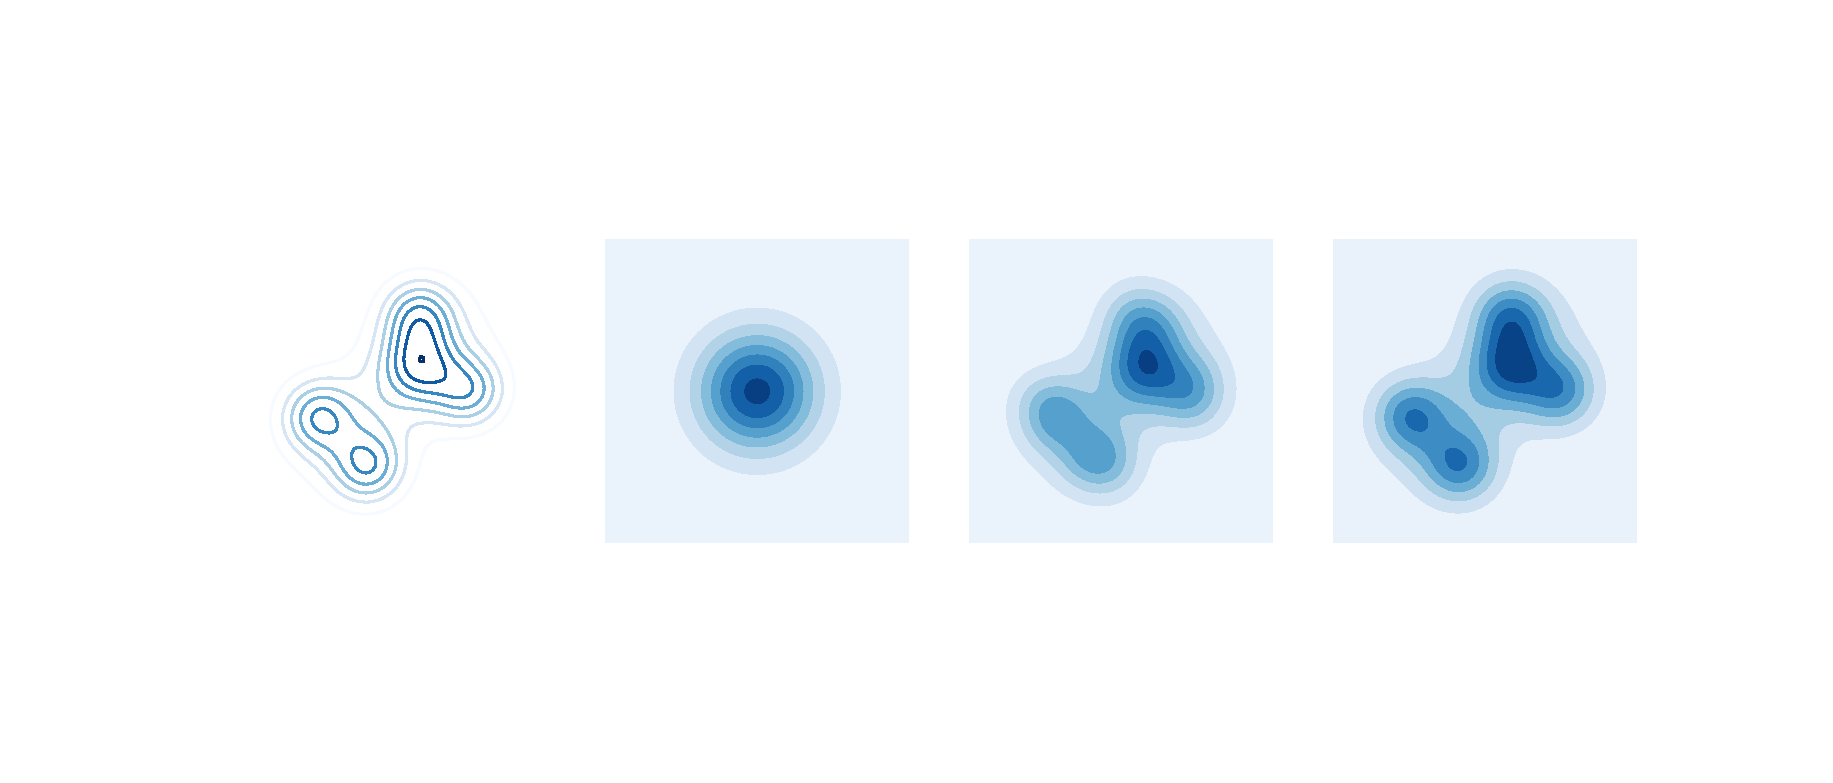
\includegraphics[width=18in]{figure_1.eps}
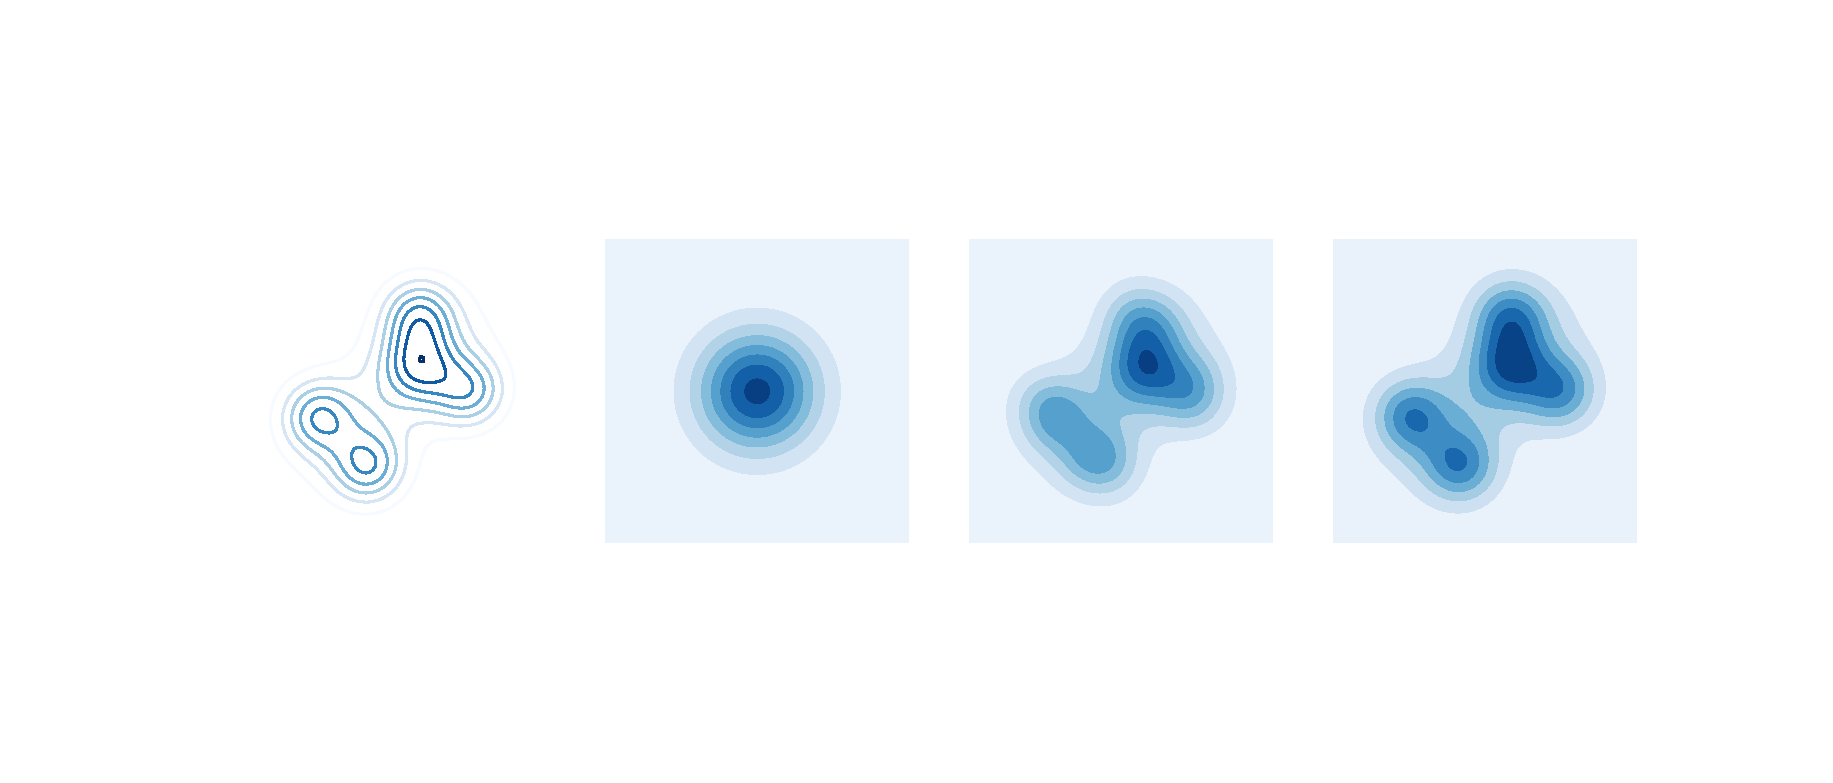
\includegraphics[width=18in, clip, trim=2.5cm 3.9cm 2cm 3.6cm]{figure_1.eps}
\end{center}
\end{textblock}











\begin{textblock}{10}(24,18)
\CHead{Resampling for Prediction}
\vspace{-1mm}
\hrule
\vspace{3mm}
During training, we sample the $q$ distribution and implicitly weight them with the IWAE ELBO. After training, we need to explicitly reweight samples from $q$.\vspace{5mm}\\
\vspace{5mm}
\normalsize{Real \qquad Sample $q(z|x)$  \qquad \qquad Sample $q_{IW}(z|x)$}
\vspace{-3mm}
\begin{figure}[h]
  \centering
      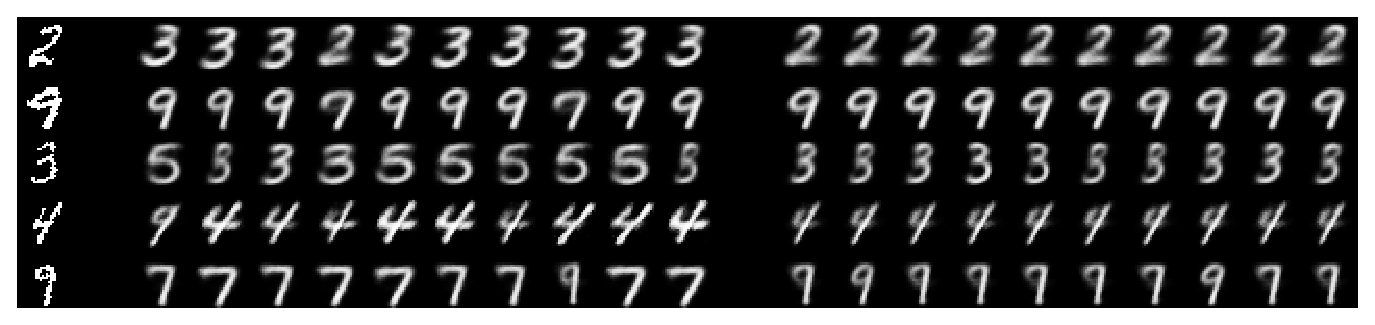
\includegraphics[width=8in, clip, trim=0cm 0cm 0cm 0cm]{recon_samplingiwae.eps}
%   \caption{Reconstructions of MNIST samples from $q(z|x)$ and $q_{IW}$. The model was trained by maximizing the IWAE ELBO with K=50 and 2 latent dimensions. The reconstructions from $q(z|x)$ are greatly improved with the sampling-resampling step of $q_{IW}$.}
%   \label{recon}
\end{figure}
\vspace{5mm}

The above figure demonstrates the need to sample from $q_{IW}$ rather than $q(z|x)$ for reconstructing MNIST digits. We trained the model to maximize the IWAE ELBO with K=50 and 2 latent dimensions. When we reconstruct samples from $q(z|x)$, we see a number of anomalies. However, if we perform the sampling-resampling step, then the reconstructions are much more accurate. The intuition here is that we trained the model with $q_{IW}$ with $K=50$ then sampled from $q(z|x)$ ($q_{IW}$ with $K=1$).
\end{textblock}















\begin{textblock}{10}(36,04)
\CHead{Discussion}
\hrule
\vspace{3mm}
The standard interpretation of importance-weighted autoencoders is that they maximize a tighter lower bound on the marginal likelihood.
We give an alternate interpretation of this procedure: that it optimizes the standard variational lower bound, but using a more complex distribution. In other words, the IWAE lower bound can be interpreted as the standard VAE lower bound with an implicit $q_{IW}$ distribution. Bachman and Precup \cite{bachman} also showed that the IWAE objective is equivalent to stochastic variational inference with a proposal distribution corrected towards the true posterior via normalized importance sampling. %We build on this idea by further examining $q_{IW}$ and by providing visualizations to help better grasp the interpretation. \\
\\

In light of this, IWAE can be seen as increasing the complexity of the approximate distribution $q$, similar to other methods that increase the complexity of $q$, such as Normalizing Flows (\cite{normflow}), Variational Boosting (\cite{varboosting}) or Hamiltonian variational inference (\cite{salimans2015markov}). With this interpretation in mind, we can generalize $q_{IW}$ to be more broadly applicable to any divergence measure. An interesting avenue of future work is the comparison of IW-based variational families with alpha-divergences or operator variational objectives. 
\end{textblock}



% \begin{textblock}{10}(36,15)
% \begingroup
% \renewcommand{\section}[2]{}%
% %\renewcommand{\chapter}[2]{}% for other classes
% \bibliography{posterTemplate}
% \endgroup
% \end{textblock}


\begin{textblock}{10}(36,18)
\CHead{References}
\hrule
\vspace{3mm}
\bibliographystyle{plain}
\small{\bibliography{posterTemplate}}
\end{textblock}



% \begin{textblock}{46}(00,25.5)
% \begin{center}
% {\footnotesize Contact information:
% Anand D.~Sarwate, 264 Cory Hall, Department of EECS, University of California, Berkeley, Berkeley, CA 94720\ \ --
% Phone: 510--643--9263\ \ -- 
% Email: \textit{asarwate@eecs.berkeley.edu}; 
% Web: \textit{http://www.eecs.berkeley.edu/}
% }
% \vspace{-0.75\baselineskip}

% {\footnotesize Acknowledgments: This work was performed while the
% author held a National Defence Science and Engineering Graduate
% Fellowship.  This template was modified only slightly from that of Ron
% Kumon in order to make it more specifically a tutorial for the
% Berkeley Wireless Foundations Center.}
% \end{center}
% \end{textblock}

\end{document}
